\documentclass{standalone}
% This file was created with tikzplotlib v0.9.15.

\usepackage{siunitx}
\usepackage{pgfplots}
% and optionally (as of Pgfplots 1.3):
\pgfplotsset{compat=newest}
\pgfplotsset{plot coordinates/math parser=false}
\newlength\figureheight
\newlength\figurewidth

\newcommand{\Set}[1]{\mathcal{#1}}
\newcommand{\Vector}[1]{\bm{\MakeLowercase{#1}}}
\newcommand{\Operator}[1]{\bm{\MakeUppercase{#1}}}
%%%%%%%%%%
\DeclareMathAlphabet{\mathsfbr}{OT1}{cmss}{m}{n}%for math sans serif (cmss)
\SetMathAlphabet{\mathsfbr}{bold}{OT1}{cmss}{bx}{n}%for math sans serif (cmss)
\DeclareRobustCommand{\msf}[1]{%
  \ifcat\noexpand#1\relax\msfgreek{#1}\else\mathsfbr{#1}\fi%for math sans serif (cmss)
}
\DeclareFontEncoding{LGR}{}{} % or load \usepackage{textgreek}
\DeclareSymbolFont{sfgreek}{LGR}{cmss}{m}{n}
\SetSymbolFont{sfgreek}{bold}{LGR}{cmss}{bx}{n}
\DeclareMathSymbol{\sXi}{\mathalpha}{sfgreek}{`X}
\DeclareMathSymbol{\sUpsilon}{\mathalpha}{sfgreek}{`U}

\begin{document}

% This file was created with tikzplotlib v0.9.15.
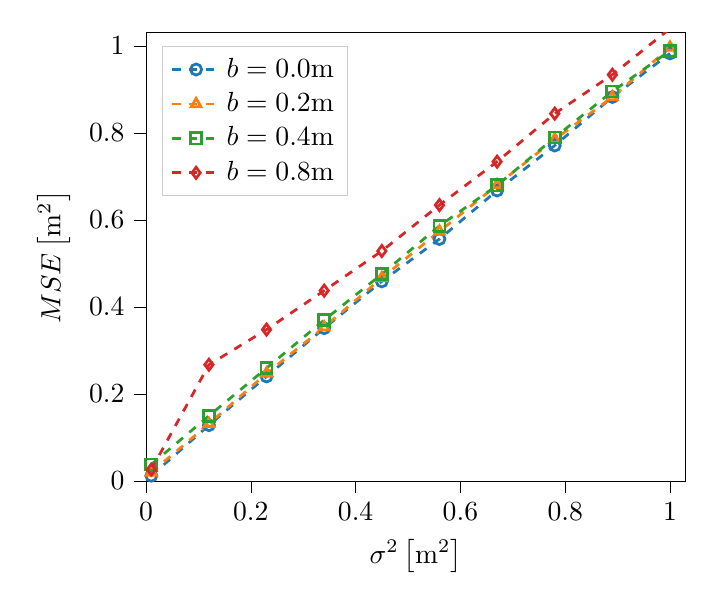
\begin{tikzpicture}

\definecolor{color0}{rgb}{0.12156862745098,0.466666666666667,0.705882352941177}
\definecolor{color1}{rgb}{1,0.498039215686275,0.0549019607843137}
\definecolor{color2}{rgb}{0.172549019607843,0.627450980392157,0.172549019607843}
\definecolor{color3}{rgb}{0.83921568627451,0.152941176470588,0.156862745098039}

\begin{axis}[
legend cell align={left},
legend style={
  fill opacity=0.8,
  draw opacity=1,
  text opacity=1,
  at={(0.03,0.97)},
  anchor=north west,
  draw=white!80!black
},
tick align=outside,
tick pos=left,
x grid style={white!69.0196078431373!black},
xlabel={$\sigma^2 \left[ \si{m^2} \right]$},
xmin=0, xmax=1.03,
xtick style={color=black},
y grid style={white!69.0196078431373!black},
ylabel={$MSE \left[ \si{m^2} \right]$},
ymin=0, ymax=1.03,
ytick style={color=black}
]
\addplot [dashed, semithick, color0, line width=1, mark=o, mark options={solid, color0}, mark repeat=1]
table {%
0.01 0.01235525
0.12 0.12840825
0.23 0.24041425
0.34 0.351263
0.45 0.4587535
0.56 0.5560815
0.67 0.667568
0.78 0.770878
0.89 0.882334
1 0.982519
};
\addlegendentry{$b = 0.0 \si{m}$}
\addplot [dashed, semithick, color1, line width=1, mark=triangle, mark options={solid, color1}, mark repeat=1]
table {%
0.01 0.01999875
0.12 0.13161325
0.23 0.24741125
0.34 0.35342025
0.45 0.466717
0.56 0.57367
0.67 0.68026575
0.78 0.784943
0.89 0.88216975
1 0.99640175
};
\addlegendentry{$b = 0.2 \si{m}$}
\addplot [dashed, semithick, color2, line width=1, mark=square, mark options={solid, color2}, mark repeat=1]
table {%
0.01 0.0380225
0.12 0.1499265
0.23 0.2595525
0.34 0.3699065
0.45 0.4755225
0.56 0.586331
0.67 0.67940425
0.78 0.7893475
0.89 0.89504675
1 0.98882275
};
\addlegendentry{$b = 0.4 \si{m}$}
\addplot [dashed, semithick, color3, line width=1, mark=diamond, mark options={solid, color3}, mark repeat=1]
table {%
0.01 0.026337
0.12 0.2672855
0.23 0.34805575
0.34 0.437537
0.45 0.52854925
0.56 0.63409475
0.67 0.73380525
0.78 0.8441835
0.89 0.93363425
1 1.03948425
};
\addlegendentry{$b = 0.8 \si{m}$}
\end{axis}

\end{tikzpicture}

\end{document}